\subsection{Learning Social Behaviour from Wizards}
\label{subsec:RestrictedPerceptionsWOZStudy}

More recently, researchers are proposing to use \ac{WoZ} studies to train virtual agents~\cite{Knox2014, Mutlu2006}. In \ac{WoZ} studies~\cite{Steinfeld2009}, subjects are led to believe that they are interacting with an autonomous robot when, in fact, they are interacting with a human (the wizard). However, when applying \ac{WoZ} in learning environments~\cite{Knox2014}, robots possess limitation and constraints over their perceptions and actions that the human expert (the wizard) does not have. For this matter, Sequeira et al., developed a novel approach, based on \ac{WoZ}, that restricts the wizard's perceptions over the environment and the behaviours it controls according to the agents' inherent limitations.

\paragraph{\textbf{Procedure Description}}

Following Figure~\ref{fig:RestrictedPerception_DesignProcess}, the development design is separated into three stages: \textit{Data Collection}, \textit{Strategy Extraction}, and \textit{Strategy Refinement}.

In the first stage, \textit{Data Collection}, mock-up studies are conducted to gain expert knowledge of common patterns in the target scenario. From the collected information, the set of all perceptions and possible actions (shared between the agent and the wizard) will define the \textit{Task AI} module.

From the previous mockup and \ac{WoZ} studies, in the \textit{Strategy Extraction} stage, a \textit{Hybrid Controller} that will guide interactions is developed, containing:
\begin{itemize}
	\item \textbf{\textit{Rule-based module}}: defines high-level interactional rules that are triggered by simpler perceptual. E.g., summarise student's progress at the ending of the session;
	\item \textbf{\textit{\ac{ML}-based module}}: using \ac{ML} classifiers, it handles more complex situations, that may emerge during the sessions, that are harder to specify using behaviour rules.
\end{itemize}

The \textit{Hybrid Controller} has the same responsibilities as the wizard: deciding when and which behaviour to trigger.

In the last stage, \textit{Strategy Refinement}, \ac{HRI} researchers evaluates the generated interaction strategies to refine the agent's behaviours for situations that may not have been properly learned or, for situations that require more relevant information.

\begin{figure}
	\centering
	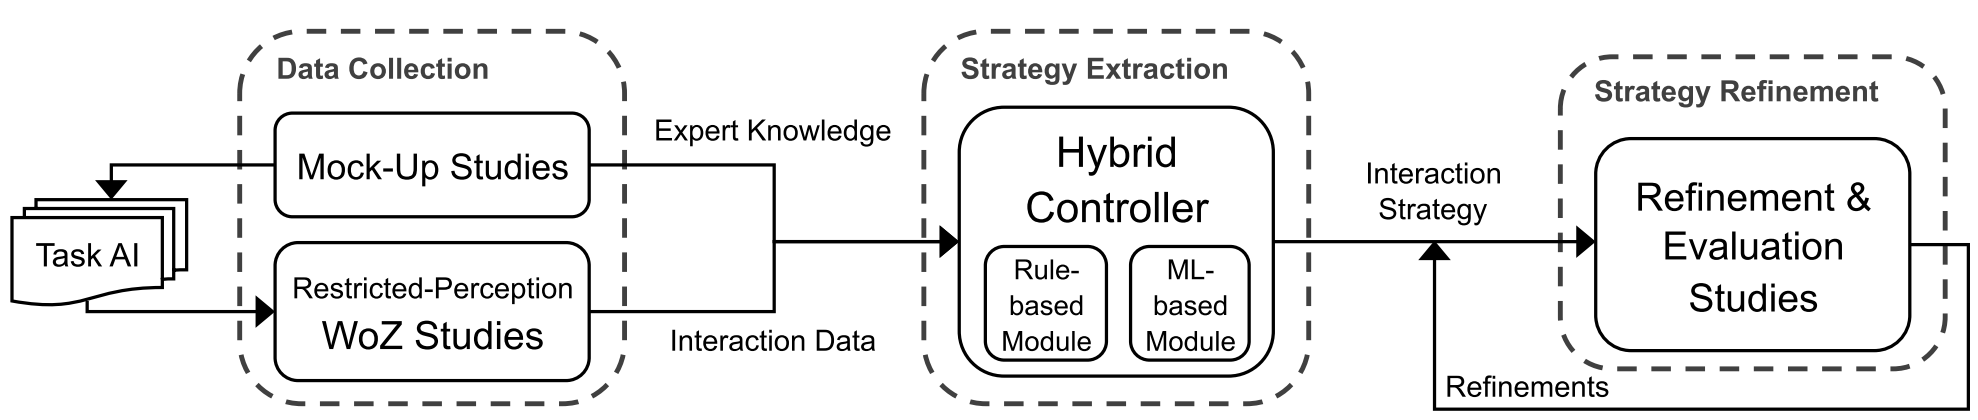
\includegraphics[width=\textwidth]{images/RestrictedPerception_DesignProcess.png}
	\caption{Different stages of the methodology for discovering interaction strategies from restricted-perception \ac{WoZ} studies. From~\cite{Sequeira2016}.}
	\label{fig:RestrictedPerception_DesignProcess}
\end{figure}

%%%%%%%%%%%%%%%%%%%%%%%%%%%%%%%%%%%%%%%%%%%%%%%%%%%%%%%%%%%%%%%%%%%%%%%%%%%%%%%%%
%%%%%%%%%%%%%%%%%%%%%%%%%%%%%%%%%%%%%%%%%%%%%%%%%%%%%%%%%%%%%%%%%%%%%%%%%%%%%%%%%
%%%%%%%%%%%%%%%%%%%%%%%%%%%%%%%%%%%%%%%%%%%%%%%%%%%%%%%%%%%%%%%%%%%%%%%%%%%%%%%%%

\paragraph{\textbf{Evaluation}}

The proposed methodology was tested using a autonomous humanoid tutor capable of learning with young learners in a multiplayer turn-based collaborative video game for building sustainable cities~\cite{Ribeiro2014}. The authors compare the fully-autonomous hybrid controller and a standard unrestricted \ac{WoZ} robot regarding empathy using \ac{IRI}~\cite{Davis1980}, anthropomorphism, animacy, likeability, perceived intelligence and perceived safety of robots using Godspeed series~\cite{Bartneck2009}, and engagement using task-related questionnaires.

%%%%%%%%%%%%%%%%%%%%%%%%%%%%%%%%%%%%%%%%%%%%%%%%%%%%%%%%%%%%%%%%%%%%%%%%%%%%%%%%%
%%%%%%%%%%%%%%%%%%%%%%%%%%%%%%%%%%%%%%%%%%%%%%%%%%%%%%%%%%%%%%%%%%%%%%%%%%%%%%%%%
%%%%%%%%%%%%%%%%%%%%%%%%%%%%%%%%%%%%%%%%%%%%%%%%%%%%%%%%%%%%%%%%%%%%%%%%%%%%%%%%%

\paragraph{\textbf{Discussion}} 

The results showed that empathy was perceived similarly between all conditions but the unrestricted \ac{WoZ} interaction strategies were preferred. The perceived intelligence and security were slightly higher in the restrictive \ac{WoZ}, and the restricted-perception \ac{WoZ} based robots were able to engage very naturally in socially-aware interactions.

This approach requires more preparation than the unrestricted \ac{WoZ} and, as the author suggests, even by using restrictive \ac{WoZ}, it is difficult to isolate the human expert's implicit knowledge regarding the environment.

To conclude, the most important aspects that may contribute to the proposed solution are:
\begin{itemize}
	\item Use of mockup-studies to gain preliminary insight of common patterns in human behaviour;
	\item Restricting the wizard's perceptions to the same extent as the agent;
	\item Use of an iterative approach to further refine the model in each iteration;
	%\item Usage of lazy learning to reduce overfitting issues;
	\item Hybrid controller with rule-based and \ac{ML}-based modules for simple and more complex perceptual states, respectively;
	\item Usage of thinking aloud technique to gain further insight on the users~\cite{Nielsen1992}.
\end{itemize}